\section{Validation and Application}

\subsection{Setup}


\begin{figure}
    \centering
    \resizebox{\linewidth}{!}{% Resize table to fit within
    
    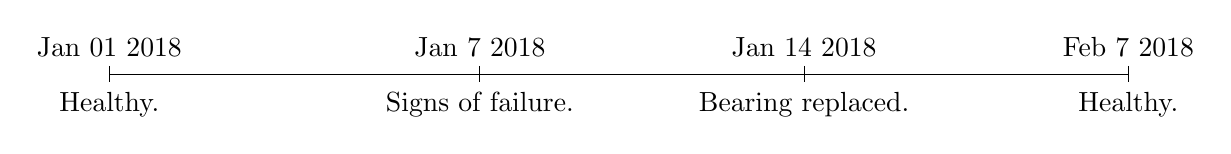
\begin{tikzpicture}[]
    %draw horizontal line
    \draw (0,0) -- (22/1.7,0);
    %draw vertical lines
    \foreach \x in {0, 8, 15, 22}{
       \draw (\x/1.7,3pt) -- (\x/1.7,-3pt);
    }
    %draw nodes
    \draw (0,0) node[below=3pt] { Healthy. } node[above=3pt] { Jan 01 2018  };
    \draw (8/1.7,0) node[below=3pt] { Signs of failure. } node[above=3pt] { Jan 7 2018  };
    \draw (15/1.7,0) node[below=3pt] { Bearing replaced. } node[above=3pt] { Jan 14 2018  };
    \draw (22/1.7,0) node[below=3pt] { Healthy. } node[above=3pt] { Feb 7 2018  };
    \end{tikzpicture}
    }
    \caption{Time Line}
    \label{fig:time_line}
\end{figure}

Four data sets were received representing two weeks, one week, the day of, 
and three weeks after a bearing failure occurred \ref{fig:time_line}.
Each data set has data sampled at an interval of 0.2 milliseconds, although data values are only updated every two milliseconds or so.
After talking to a subject matter expert, it was determined that the data one week and the day of should be considered as failing.
The data two weeks before and three weeks after represent healthy data.
Therefore the experiment setup is as follows:
\begin{enumerate}
    \item the SOM will be trained on data from February 7th.
    \item validation on January 1st data should not show signs of failure, otherwise the model failed to generalize.
    \item evaluation on January 7th and 14th should show signs of failure.
\end{enumerate}


%\begin{figure}
%    \centering
%    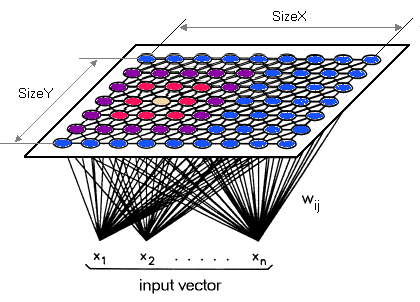
\includegraphics[scale=0.5]{som-struct}
%\end{figure}

% describe SOM map
The size of the map was set to be 64, representing a 2D grid 8 by 8 grid of neurons.
Figure \ref{fig:colourmap} shows the SOM after training the map on data from February 7th, where each square represents a neuron. 
The colour indicates how similar neighbouring neurons are, and the number of times a neuron has won a competition is labelled on each neuron.
Neurons with less than two wins are determined to be too noisy for use in the evaluation \cite{som-1}.
These neurons are ignored.
To calculate the health score, the minimum quantization error is averaged over the three closest neurons.
This is analogous to the 3-NN method used by \cite{Tian2014AnomalyDU}.
% this should be explained in detail in previous section but numbers shown here

\begin{figure}[!h]
    \centering
    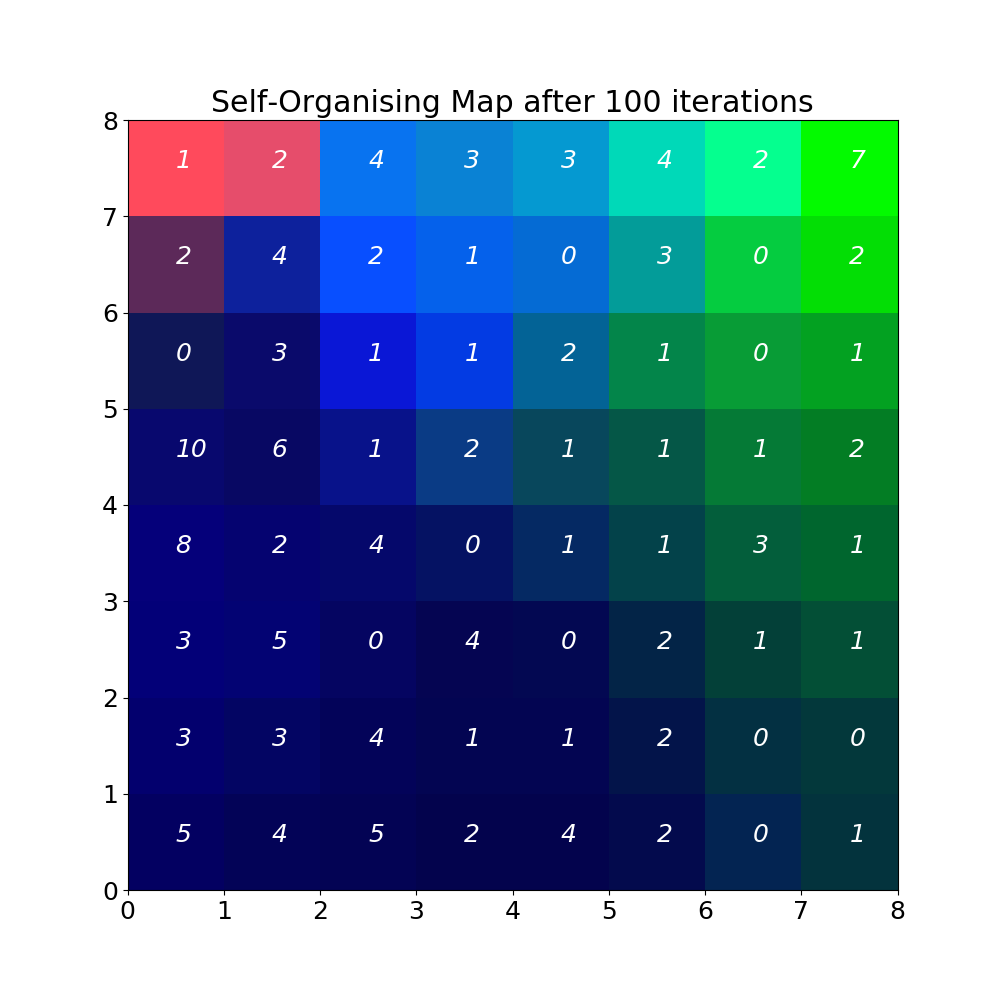
\includegraphics[width = 0.5\linewidth]{som-colour-map}
    \caption{SOM colour map showing the number of hits for each neuron in the map on the training data.}
    \label{fig:colourmap}
\end{figure}

\subsection{Results}

Operators currently analyze the vibration signals manually.
A vibration expert spends time looking at the raw vibration signals to determine a threshold.
If the threshold is crossed, an alarm is generated.
Operators must manually determine when to replace the bearing based the percentage of time spent above the threshold.
This is a common technique used in a multitude of industries.
The moving average or the standard deviation of the raw signal can also be used.
This method is compared with the SOM and the results are summarized in Table \ref{tbl:percent}.
For all methods the threshold was optimized to get the best results.
Another significant metric to compare the practicality of all methods is the number of alarms generated (see Table \ref{tbl:alarms}).
Ideally, an alarm should trigger only once to indicate failure.

The results of the health score are shown in Figure \ref{fig:health}.
The health score given by the SOM was significantly higher when operators said the bearing was failing.
Upon examination the health scores seemed to act as a smoothing mechanism for the raw vibration signal.
This makes sense intuitively as the primary determinant for a bearing's health should be the vibration signal itself.
% lots figures and explain them thoroughly
\begin{table}[!h]
    \centering
    \caption{Percentage of Time Spent Above Threshold for Each Score}
    \begin{tabular}{|c|l|l|l|}
        \hline
                                          & \multicolumn{3}{c|}{\% of Time Above Threshold } \\ \hline
                                          Method                            & January 1st             & January 7th                & January 14th               \\ \hline \hline
                                          Raw Vibration              & 0 \%              & 31.3 \%           & 34.7 \%            \\ 
        Moving. Avg.             & 0 \%               & 50.7 \%             & 47.2 \%             \\
        Moving Std. Dev. & 0 \%               & 57.5 \%             & 38 \%               \\
        SOM                               & 3.5 \%               & 100 \%                & 100 \%                \\ \hline 
    \end{tabular}
    \label{tbl:percent}
\end{table}

\begin{table}[!h]
    \centering
    \caption{Number of Times the Threshold is Crossed for Each Score}    
    \begin{tabular}{|c|l|l|l|}
        \hline
                                          & \multicolumn{3}{c|}{ (No. of Alarms) } \\ \hline
                                          Method                            & January 1st             & January 7th                & January 14th               \\ \hline \hline
        Raw Vibration              & 1               & 5630            & 5975           \\ 
        Moving Avg.             & 1               & 380             & 204             \\ 
        Moving Std. Dev. & 1              & 370             & 206               \\ 
        SOM                               & 1               & 1               & 1                \\ \hline
    \end{tabular}
    \label{tbl:alarms}
\end{table}

\begin{figure}[!h]
    \centering
    \begin{subfigure}{6cm}
        \centering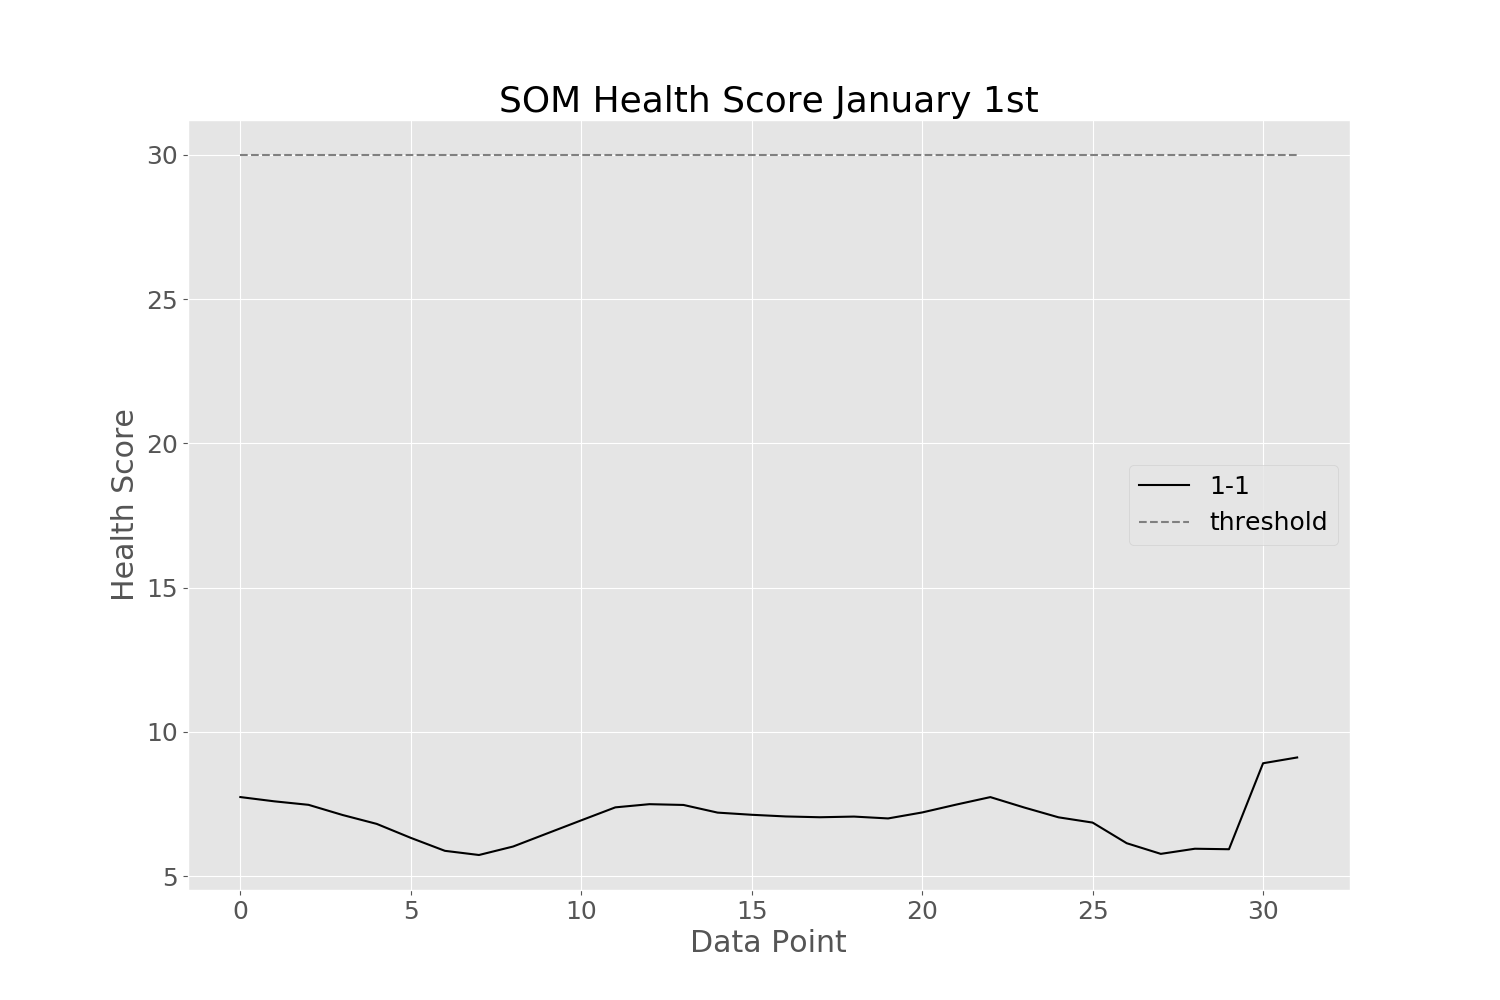
\includegraphics[trim={300 50 50 50}, width=\linewidth]{health_score-jan1}
    \end{subfigure}%
    \begin{subfigure}{6cm}
        \centering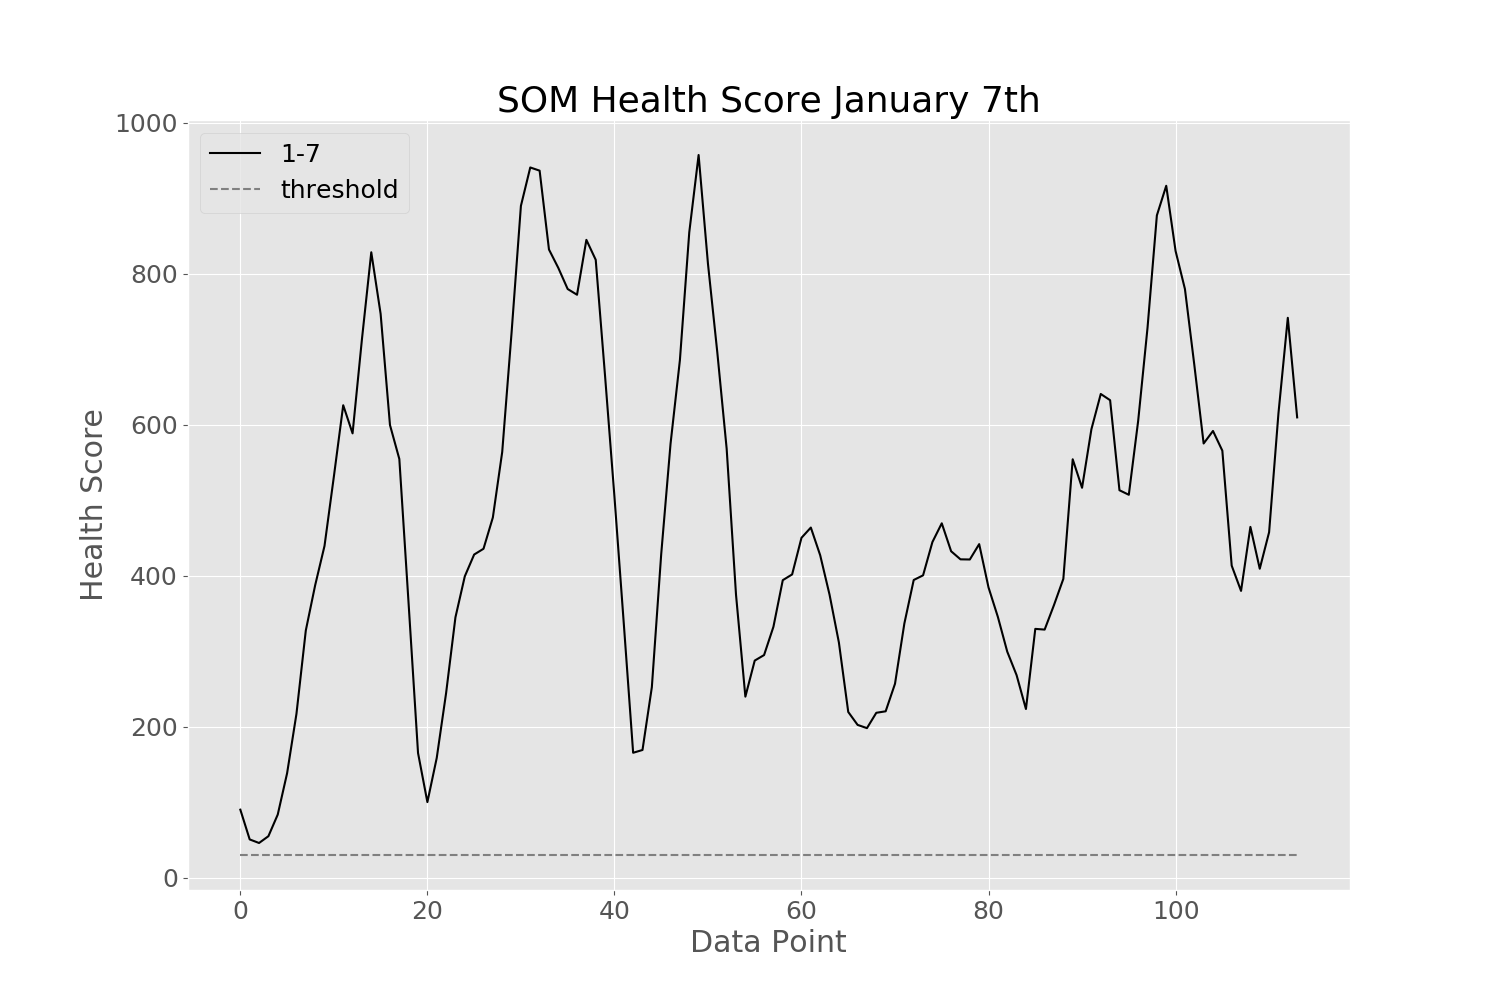
\includegraphics[trim={50 50 300 50}, width=\linewidth]{health_score-jan7}
    \end{subfigure}\vspace{10pt}
 
    \begin{subfigure}{6cm}
        \centering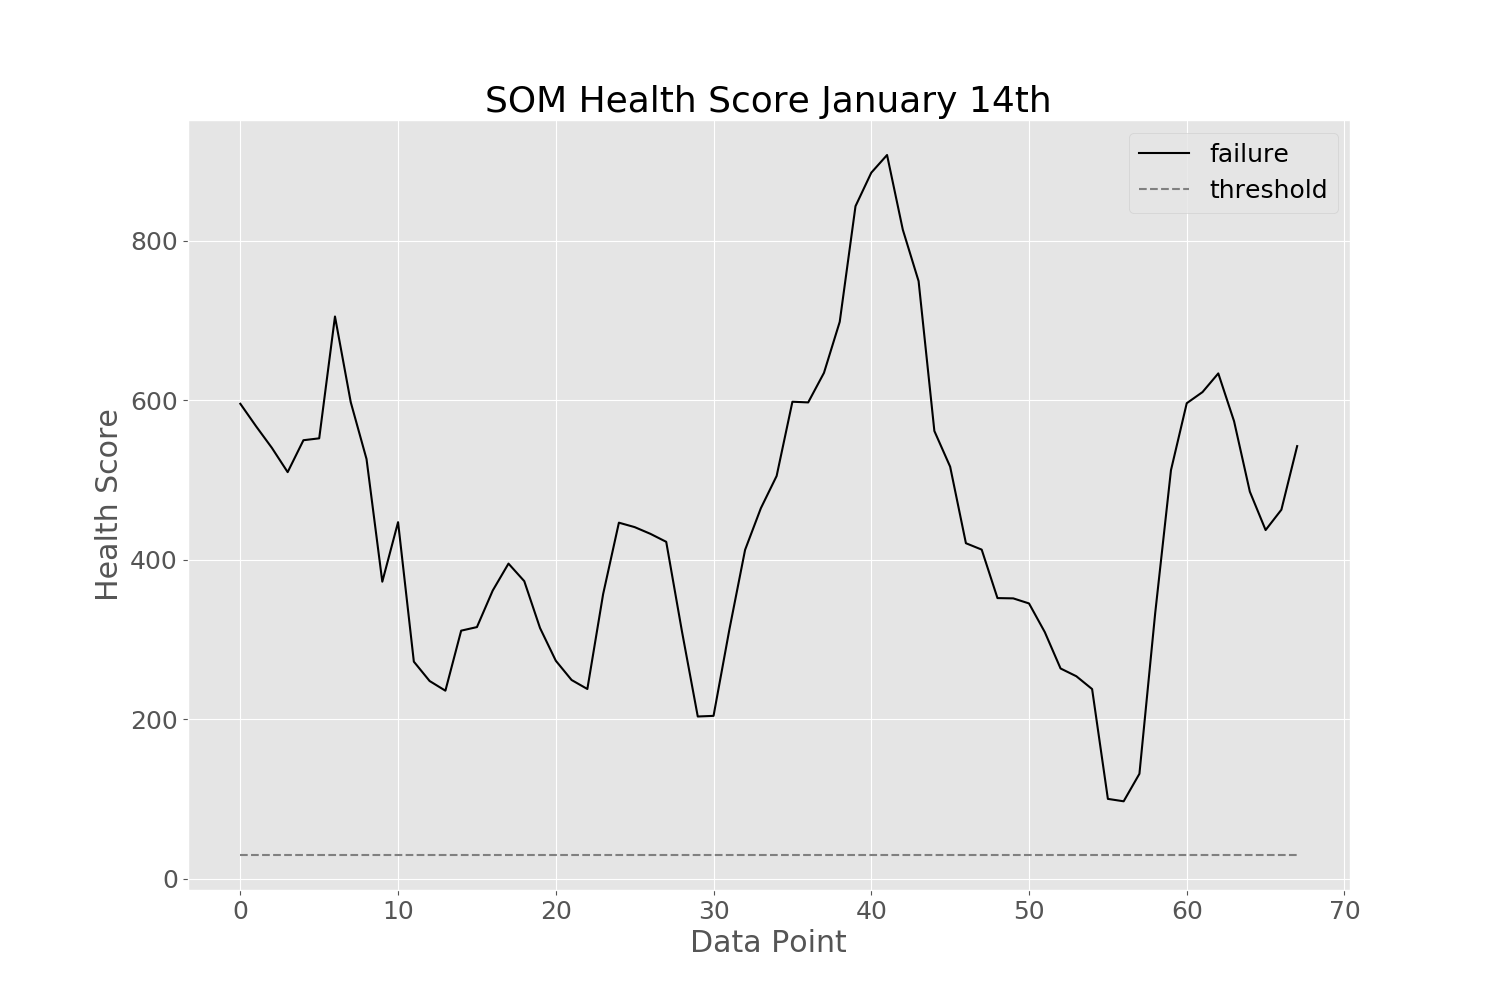
\includegraphics[trim={300 50 50 50}, width=\linewidth]{health_score-jan14}
    \end{subfigure}%
    \begin{subfigure}{6cm}
        \centering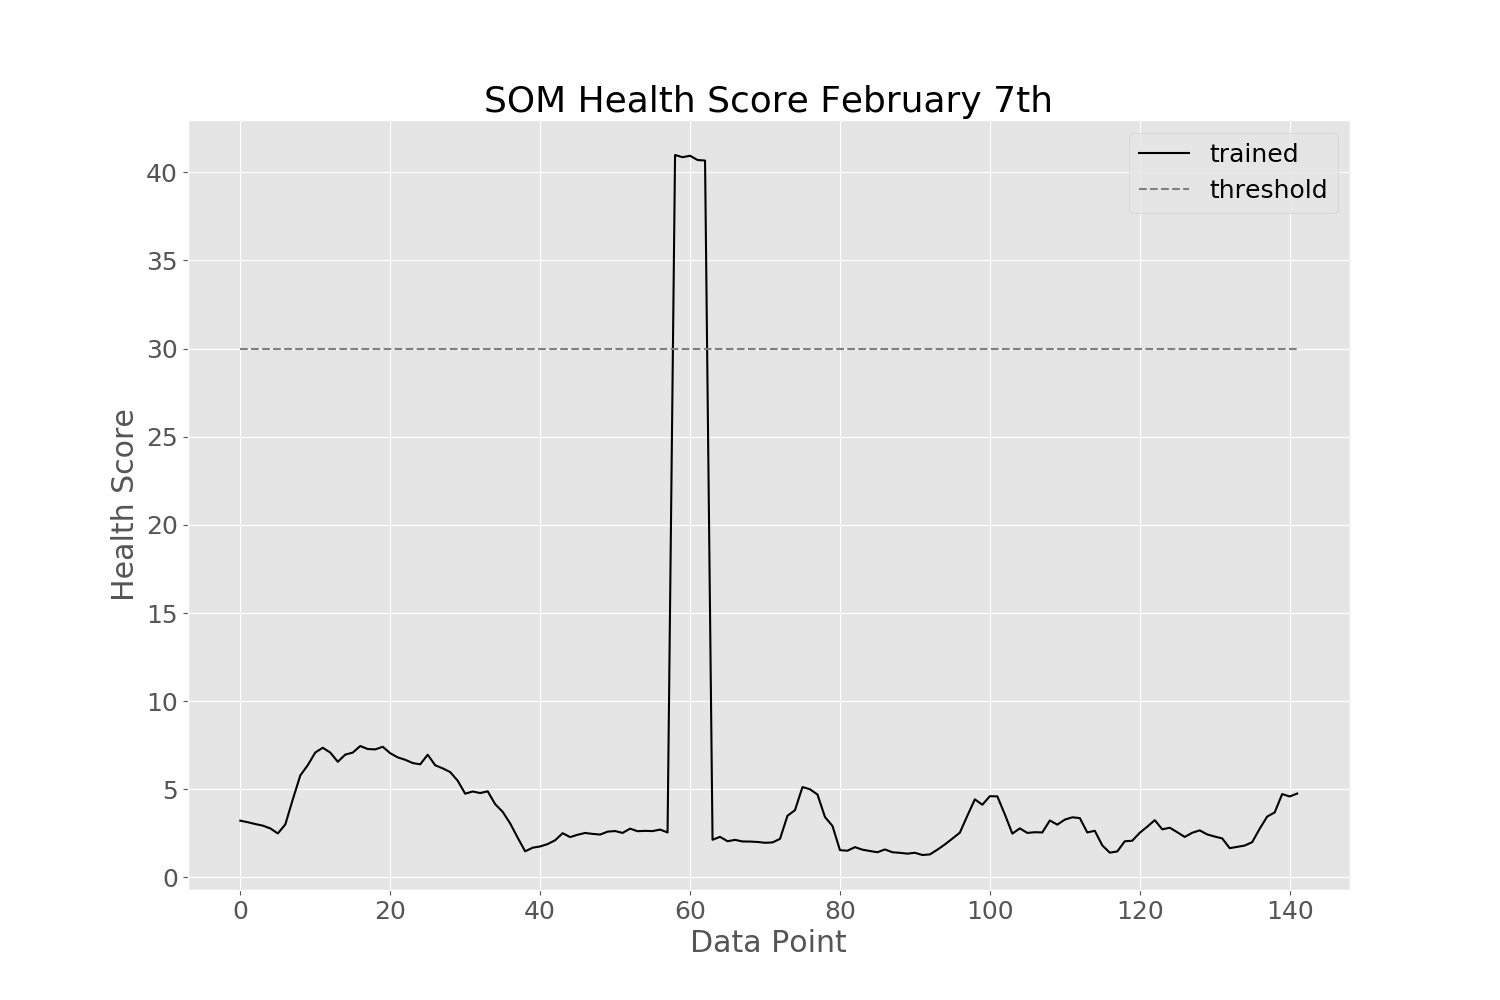
\includegraphics[trim={50 50 300 50}, width=\linewidth]{health_score-feb7}
    \end{subfigure}
    \caption{Bearing health scores for each data set. The threshold is set to 30. The SOM map is able to smooth the raw vibration signal to provide a robustness health metric.}
    \label{fig:health}
\end{figure}
